\chapter{HyperSpy quantification}
\label{appendix:HSquant}

The following notebook is quantification in HyperSpy.
The notebook does three quantifications: linear background removal and intensities from the raw spectrum, intensities from a fitted model, and intensities from a model fitted with calibration in HyperSpy.

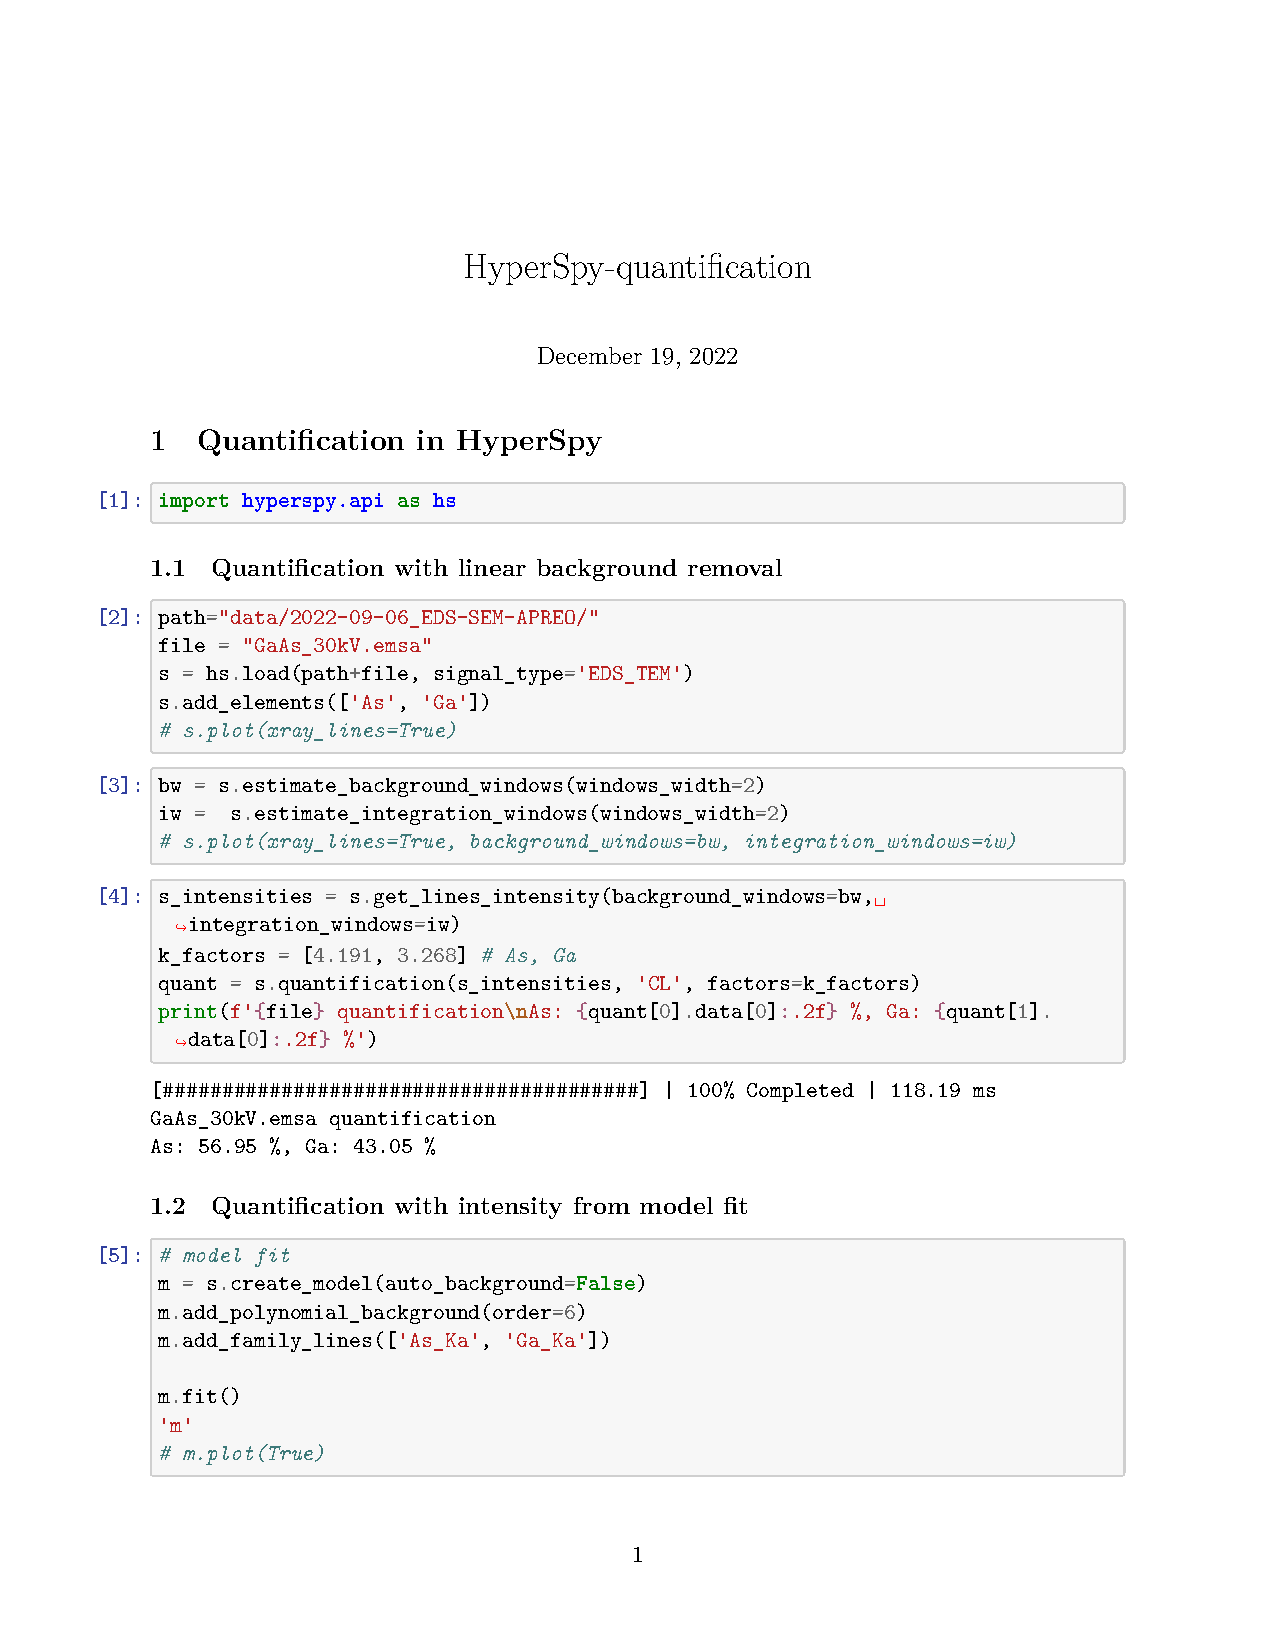
\includepdf[pages=-,pagecommand={},width=\textwidth]{chapters/HyperSpy-quantification.pdf}



\chapter{Peak and background modelling}
\label{appendix:modelling}

This is a notebook for calibration.
The calibration is done on the 30 kV spectrum of GaAs bulk.

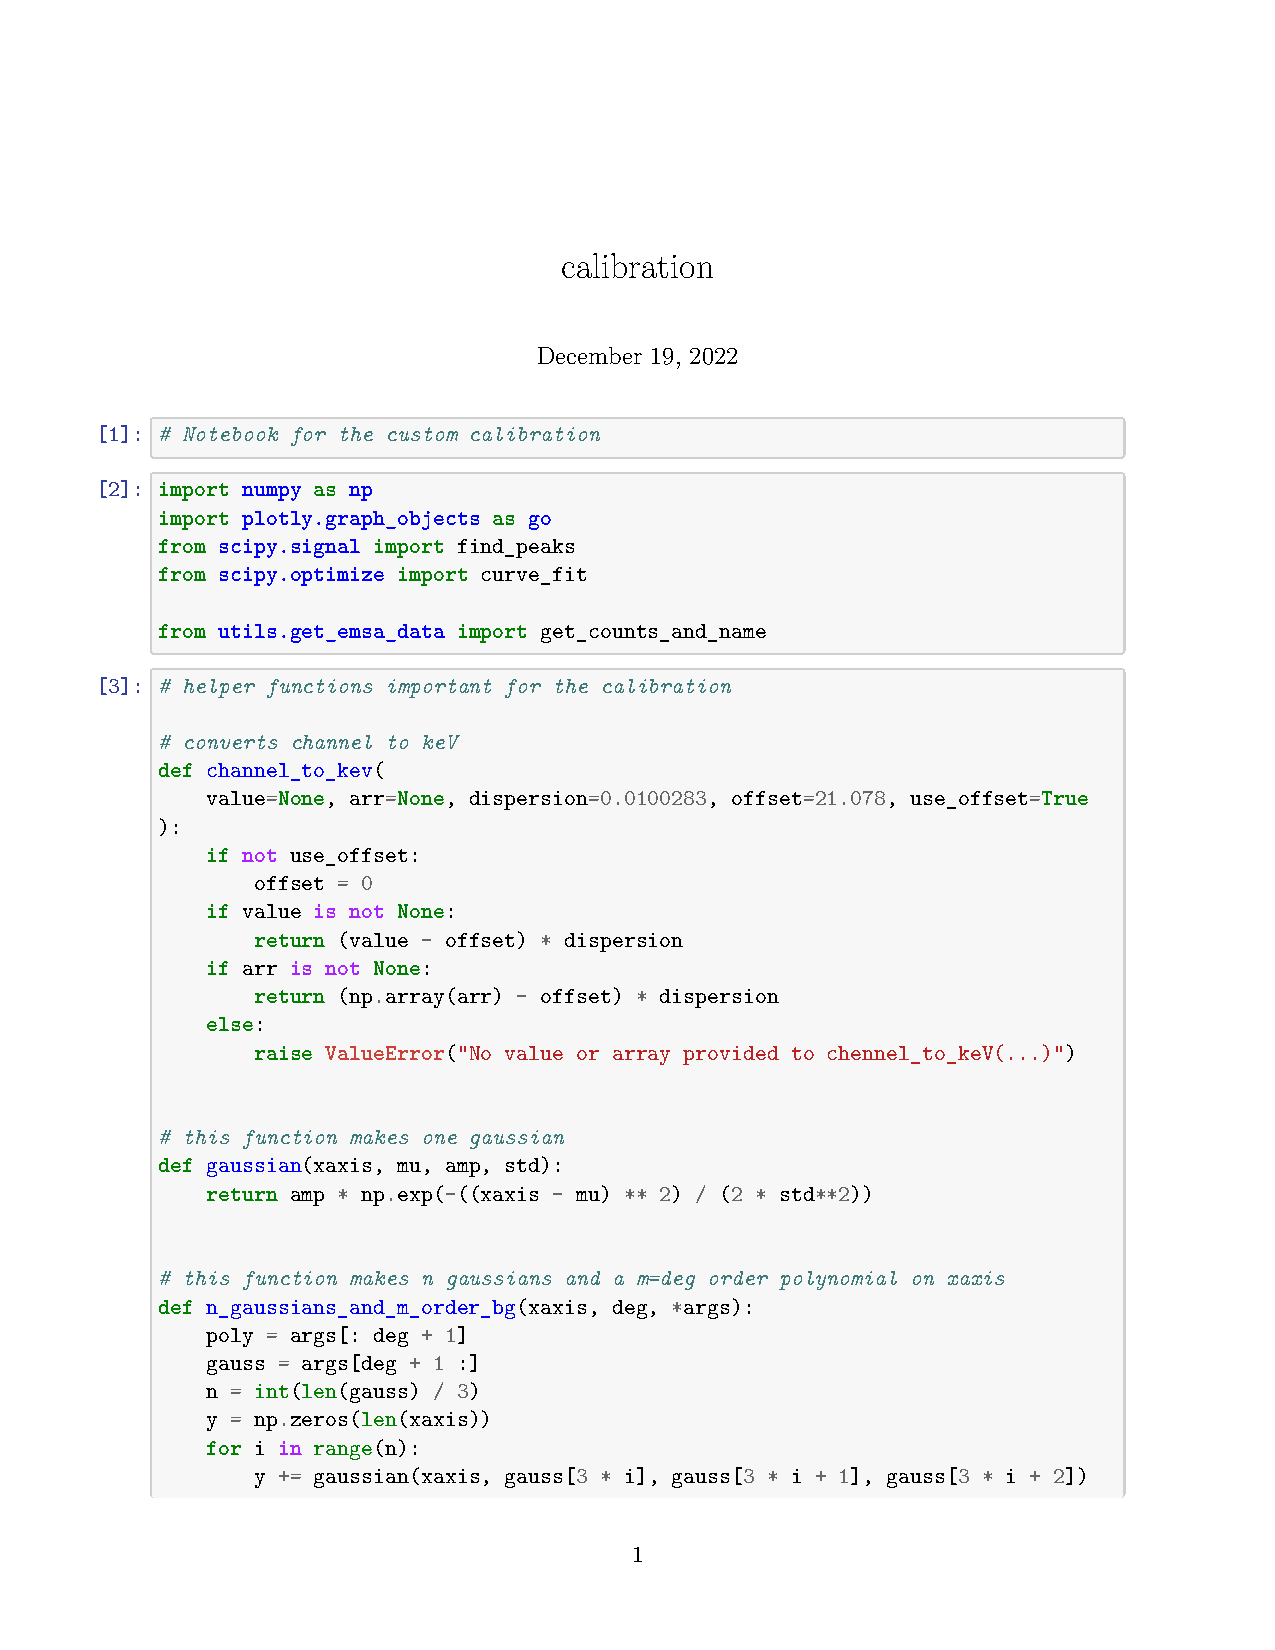
\includepdf[pages=-,pagecommand={},width=\textwidth]{chapters/calibration.pdf}


% \chapter{Plotly plotting}
% \label{appendix:plotting}

% Insert description.

% Insert the code here.